
\graphicspath{ {5chapterImplementation/image/} }
\chapter{Implementation}

This chapter will clarify the implementation of the approach present in \autoref{Approach}. 
\section{Gray-level conversion and well-composed interpolation}
First of all, the color input images will be transformed into gray level image using its luminance information. Most digital images using the RGB (or sRGB) which use the ITU-R BT.709 primaries. The coefficients defined to calculate the relative luminace from linear RGB components is: $Y = 0.2126R + 0.7152G + 0.0722B$. The formula reflects the spectral sensitivity of human visual perception of brightness: green light contributes the most to the intensity perceived by humans, and blue light the least. Other steps will work on this image. 
\par At first, morphological Laplacian is calculated using a relatively large size structuring element to reduce influences of small components. A morphological gradient will also be calculated to provide information for pruning the tree \textit{a priori}. These output images will be doubled the resolution using a well-composed Interpolation \fxnote{add more detail}

\par The topology of the output images are not well-composed and therefor does not provide the self-dual \fxnote{why we have to interpolate}. Our method will double the resolution of the image by a well-composed interpolation. This interpolation will add temporary points:
\par
\begin{table}
	\centering
	\begin{tabular}{|c|c|c|}
	\hline 
	a & ${(a+b)}/{2}$ & b \\ 
	\hline 
	${(a+c)}/{2}$ & $median(a,b,c,d)$ & ${(b+d)}/{2}$ \\ 
	\hline 
	c & ${(c+d)}/{2}$ & d \\ 
	\hline 

	\end{tabular}
	\caption{Well-composed interpolation} 
\end{table}

\par
As proved in \cite{geraud.15.ismm}, if added points is calculate by the median of points around them will leads to a self-dual plain map.


\section{Objects labeling}

\subsection{Labeling by front propagation}
\par From the well-composed interposed laplacian, we will label all connected components by front propagation. A connected component contain a set of connected pixels that has same sign of Laplacian and zeros that included in that region. As the zeros on the contours is always include in the outer region, we treat connected component in a dual-way i.e this process applied to complement image will gives the same result. Thanks for the well-composed interpolation, we can use only one type of connectivity. We chose the the 4-connectivity to reduce number of neighbors needed to be checked . As there are only 2 type of component (positive and negative one), a region is always surrounded by one other region. With the labeled image, we will present the tree structure with a parent table which tell the parent of each label. The parent of the root will be itself.
\par
Because of large number of component extracted by the Laplacian, we will try to prune the tree at the same time of labeling. Whenever we found a new component, some criteria will be check first to decide if a new label will be spread or continue using the label of that component's parent. These criteria includes average gradient of points on the outer contour and the perimeter of that contour.  
\par
The labeling algorithm is a modified front propagation algorithm. At first, an all zeros images is create with the same size like the interpolated Laplacian. Then the output images is read from left to right, top to bottom. For every point which is not labeled (i.e maintain the null value), a new component is detected and a label will be propagate from that point. If it is not the first point (root component), we will follow points on its boundary to calculate the average gradient and perimeter of this contour and decide if a new label will be use. If the component is small or its gradient is week, we will use its parent's label to mark this component. The label will be propagated in checking its 4 neighbors. if a neighbor is inside the image, still not labeled and having same sign of the region, it will be labeled and the label will continue propagate from that point. We continue until the component is labeled. The sign agreement can be checked simply by a xor operation between sign of region and sign of that point on the Laplacian. During the labeling process, other information can also be gather such as the bounding box, area, average gray level of each component. The pseudo code is presented in Algorithm \autoref{al:labeling}
\fxnote{pseudo code}
\par


\begin{algorithm}
\caption{labeling}\label{al:labeling}
\begin{algorithmic}[1]
\Procedure{Labeling(image,laplacian,gradient)}{}
\State $\textit{output} \gets \text{zeroes }$
\State $ level \gets 1$
\State $ boundingBox \gets image.Domain()$
\For {$\textbf{all } \textit{p}$}
\If {$output(p)$} $\textbf{continue}$
\EndIf
\If {p is the first point}
	\State $current \gets level$
	\State $tree.parent.push\_back(current)$
	\State $tree.color.push\_back(0)$
	\State $tree.area.push\_back(0)$
\Else
	\State $followEdge(p,grad,perimetre)$
	\If{\textit{grad $>$ gradThresHold} \textbf{and} \textit{perimetre $>$ perimetreThresHold}}
		\State $ level \gets level+1$
		\State $ current \gets level$
		\State $tree.parent.push\_back(current)$
		\State $tree.color.push\_back(0)$
		\State $tree.area.push\_back(0)$
		\State $tree.boundingBoxes.push\_back(boundingBox)$		
		\State $boundingBox.match(p)$
		\State $newRegionFlag \gets true$		
	\Else
		\State $current \gets output$
		\State $newRegionFlag \gets false$
	\EndIf
\EndIf

\State $output(p) \gets current $.
\State $sign\_flag \gets laplacian(p)>0$.
\State $Queue.push(p)$.

\While {\textit{Queue} \textbf{is not empty}}
	\State p $\gets$ Queue.pop()
	\State $tree.color[current-1] \gets tree.color[current-1] + image(p) $
	\State $tree.area[current-1] \gets tree.area[current-1] + 1$
	\For {$\textbf{all } \textit{neighbor of p} $}
		\If {n \textit{inside} image \textbf{and} output(n) = 0 \textbf{and} sign\_flag = laplacian(n)$ > $0}
			\State $output(n) = current$
			\State $Queue.push(n)$
			\State $boundingBox.extendToMatch(n)$
		\EndIf			
	\EndFor
\EndWhile
\EndFor
\State $tree.boundingBoxes.push\_back(boundingBox)$
\For {$i=0;i<level;i++$}
	\State tree.color[i]=tree.color[i]/tree.area[i];
\EndFor
\State \Return tree, output
\EndProcedure
\end{algorithmic}
\caption{Labeling process to construct the tree}
\end{algorithm}

\subsection{Average gradient on contour calculation}
\par We aim to prune the tree during the labeling process by merging nodes which has low contrast with the upper node which means having low gradient in the contour. By calculate average gradient of these points, we can decide which node to remove.There are many approach to obtain the contour, for example we can use a dilation follow by a erosion using a element cross as structure element to obtain the contour. But the calculation of erosion and dilation costs. Because the topology is simplified by the well-composed interpolation, which made every component is surround by only one other component, we can apply a simple contour following method to follow its outer contour.
\par As after each label propagation, component which is not yet labeled will remain null and surround by another label. For every new component detected except the first one (root), we will first follow the outer contour of the object to calculate its average gradient. As we read the image from left to right, top to bottom, first point of new region is always the left top most point of that component. 

The algorithm will try to follow the component in clockwise direction. We initialize the starting point is the one on the left of first point of component. There are 8 possible direction of next point to advance (direction are numbered as in \ref{directionToSearch}). The next point must be the one which is labeled and has a non labeled point on its left. The searching order is a semicircle clockwise from last direction plus a semicircle counter clockwise from last-direction (for example if the last direction is 0, we will check these directions in order: 0 1 2 3 7 6 5 4). We continue this until reach the starting point. The length and gradient will be gathered during the process. 

\begin{figure}
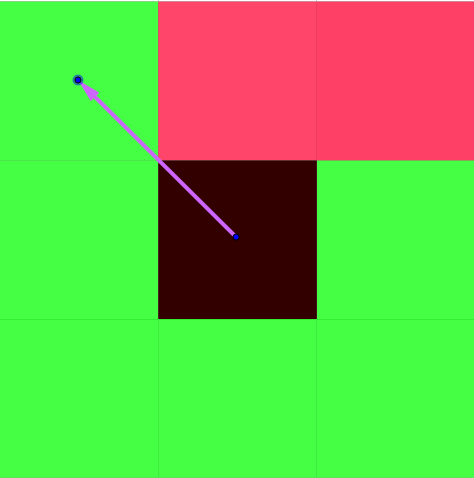
\includegraphics[width=2.5cm]{gradient/7.png}
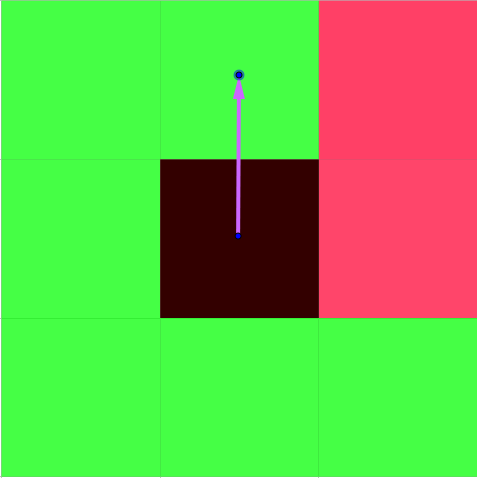
\includegraphics[width=2.5cm]{gradient/8.png}
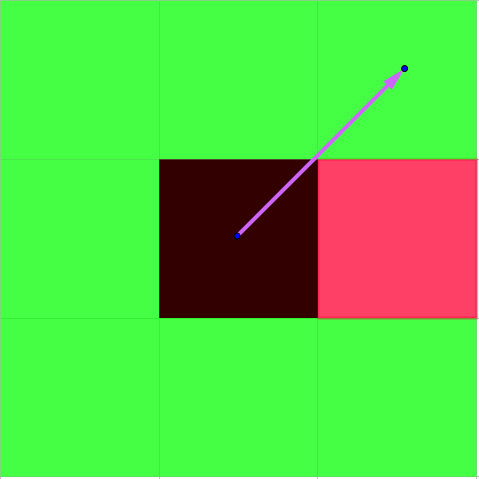
\includegraphics[width=2.5cm]{gradient/1.png}
\centering

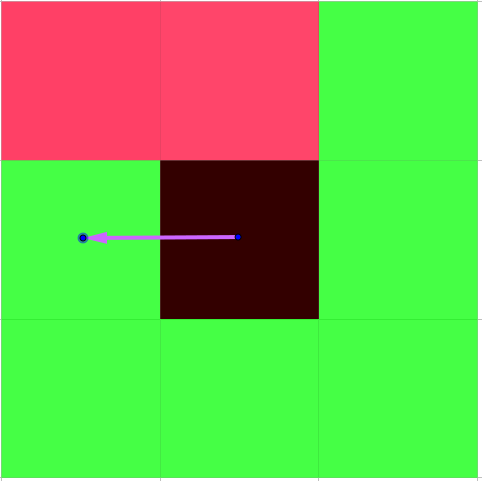
\includegraphics[width=2.5cm]{gradient/6.png}
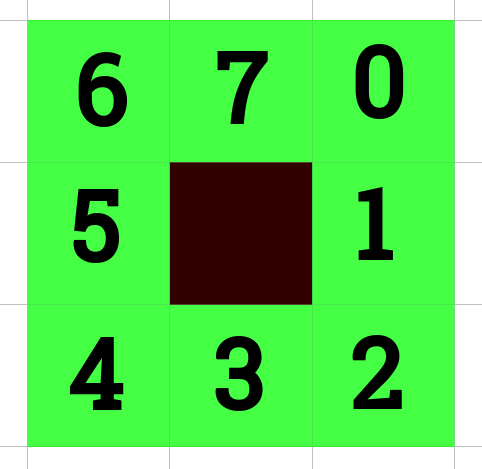
\includegraphics[width=2.5cm]{gradient/c.png}
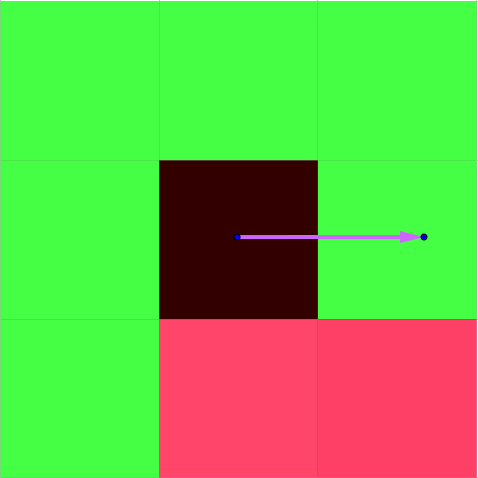
\includegraphics[width=2.5cm]{gradient/2.png}
\centering

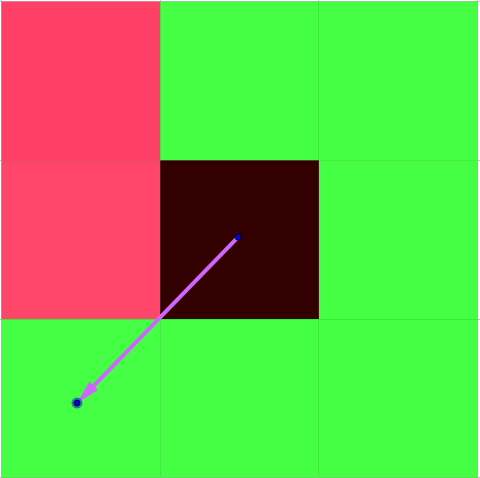
\includegraphics[width=2.5cm]{gradient/5.png}
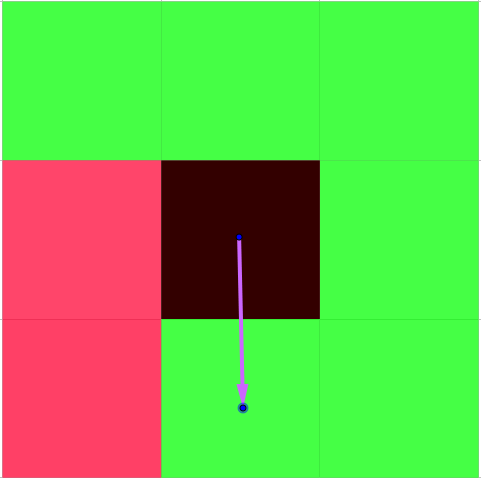
\includegraphics[width=2.5cm]{gradient/4.png}
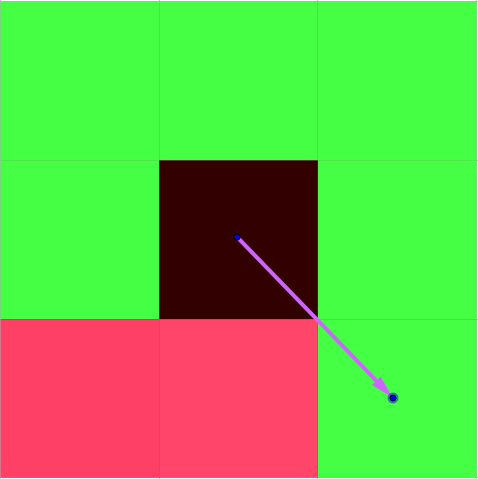
\includegraphics[width=2.5cm]{gradient/3.png}
\centering
\caption{Possible positions of next point}
\label{directionToSearch}
\end{figure}


\begin{algorithm}
\caption{FollowContour}\label{al:ContourFollowing}
\begin{algorithmic}[1]
\State $iter \gets [0,1,1,1,4,7,7,7]$
\Procedure{FollowContour(p)}{}
\State $np = p$ 
\State $count \gets 0$
\Repeat 
\For{$i=0;i<8;i++$}
	\State $direction \gets (direction + iter[i])$ \textbf{ mod 8}
	\If{$output(np+direction)!=0$ \textbf{ and } $output(np+direction+1)=0$}
		\State $np \gets np+direction$
		\State $grad \gets gradientImage(np)$
		\State $count \gets count+1$
	\EndIf
\EndFor
\Until{$np==p$}
\State $grad\gets grad/count$
\State $perimetre \gets count $
\State \Return (grad,perimeter)
\EndProcedure
\end{algorithmic}
\caption{Contour following process}
\end{algorithm}

\section{Objects labeling}